\documentclass[10pt]{article}
\usepackage{graphicx} % Required for inserting images
\usepackage[a4paper,margin=2.2cm]{geometry}
\usepackage[ruled,vlined,linesnumbered]{algorithm2e}
\usepackage[T1]{fontenc}
\usepackage[utf8]{inputenc}
\usepackage{lmodern}
\usepackage{longtable}
\usepackage{microtype}
\usepackage{amsmath,amssymb,mathtools}
\usepackage{booktabs,tabularx,array,multirow}
\usepackage{enumitem}
\usepackage{appendix}
\usepackage{booktabs}
\usepackage{array}
\usepackage{xcolor}
\usepackage{tikz}
\usepackage{enumitem}
\usepackage{amsthm}
\usetikzlibrary{arrows.meta,
positioning,
fit,
shapes.geometric, 
backgrounds, 
calc}
\usepackage{listings}
\usepackage{hyperref}
\usepackage[nameinlink,noabbrev]{cleveref}
\usepackage{caption}
\usepackage{subcaption}
\usepackage{url}
\usepackage{balance}
\usepackage{tabularx}
\usepackage{booktabs}
\usepackage{array}
\usepackage{makecell}
\usepackage{ragged2e}
\newcolumntype{C}[1]{>{\Centering\arraybackslash}p{#1}}
\newcolumntype{Y}{>{\RaggedRight\arraybackslash}X}

\definecolor{acmblue}{RGB}{37,80,130}
\definecolor{acmgray}{RGB}{245,247,249}
\definecolor{passgreen}{RGB}{34,139,34}
\definecolor{deviationorange}{RGB}{210,105,30}
\definecolor{skipgray}{RGB}{105,105,105}
\definecolor{failred}{RGB}{178,34,34}
\definecolor{alertred}{RGB}{178,34,34}
\definecolor{preservedgreen}{RGB}{34,139,34}
\definecolor{approximatedorange}{RGB}{210,105,30}
\definecolor{unsupportedgray}{RGB}{105,105,105}
\hypersetup{
  colorlinks=true,
  linkcolor=acmblue,
  citecolor=acmblue,
  urlcolor=acmblue,
  pdftitle={Agentic Configuration Management},
  pdfauthor={AUTHOR NAME}
}

\lstdefinestyle{acmcode}{
  basicstyle=\ttfamily\small,
  backgroundcolor=\color{acmgray},
  frame=single,
  rulecolor=\color{black!15},
  breaklines=true,
  columns=fullflexible,
  showstringspaces=false
}

\newcommand{\acmcore}{\textsc{ACM Core}}
\newcommand{\framework}{framework-independent}
\newcommand{\todo}[1]{\textcolor{red}{[TODO: #1]}}
\newcommand{\system}{\mathcal{S}}
\newcommand{\configgraph}{G_C}
\newcommand{\runtimegraph}{G_R}
\newcommand{\assurancegraph}{G_A}
\newcommand{\evolutiongraph}{G_E}
\newcommand{\statuspass}{\textcolor{passgreen}{\texttt{pass}}}
\newcommand{\statusdeviation}{\textcolor{deviationorange}{\texttt{pass\_with\_deviation}}}
\newcommand{\statusskip}{\textcolor{skipgray}{\texttt{skipped}}}
\newcommand{\statusfail}{\textcolor{failred}{\texttt{fail}}}
\newcommand{\statusnotexec}{\texttt{not\_executed}}
\newcommand{\statuspreserved}{\textcolor{preservedgreen}{\texttt{preserved}}}
\newcommand{\statusapproximated}{\textcolor{approximatedorange}{\texttt{approximated}}}
\newcommand{\statusunsupported}{\textcolor{unsupportedgray}{\texttt{unsupported}}}

\newtheorem{theorem}{Theorem}
\newtheorem{lemma}{Lemma}
\newtheorem{proposition}{Proposition}

\title{\textbf{Agentic Configuration Management (ACM):\\A Reference Configuration Model for Governed Agentic Systems}}

\author{
  Audrey Quessadda-Vial\\
  PwC\\
  \texttt{audrey.quessada-vial@pwc.com}
}

\date{Draft --- August 2026}

\begin{document}

\maketitle

\section{Operationalization}
\label{sec:operationalization}

The purpose of this section is not to define another execution framework but to demonstrate that the proposed reference model is operationalizable without introducing framework-specific concepts into its governance semantics. The operationalization deliberately separates governance semantics from implementation details. The ACM metamodel, lifecycle semantics, and validation rules are independent of programming language, persistence technology, communication protocol, or execution framework. The Python implementation therefore serves only as one concrete realization of the reference model, demonstrating implementability rather than prescribing a specific software architecture. The experimental methodology is depicted in Figure ~\ref{fig:experimental_protocol}.

\begin{figure*}[t]
	\centering
	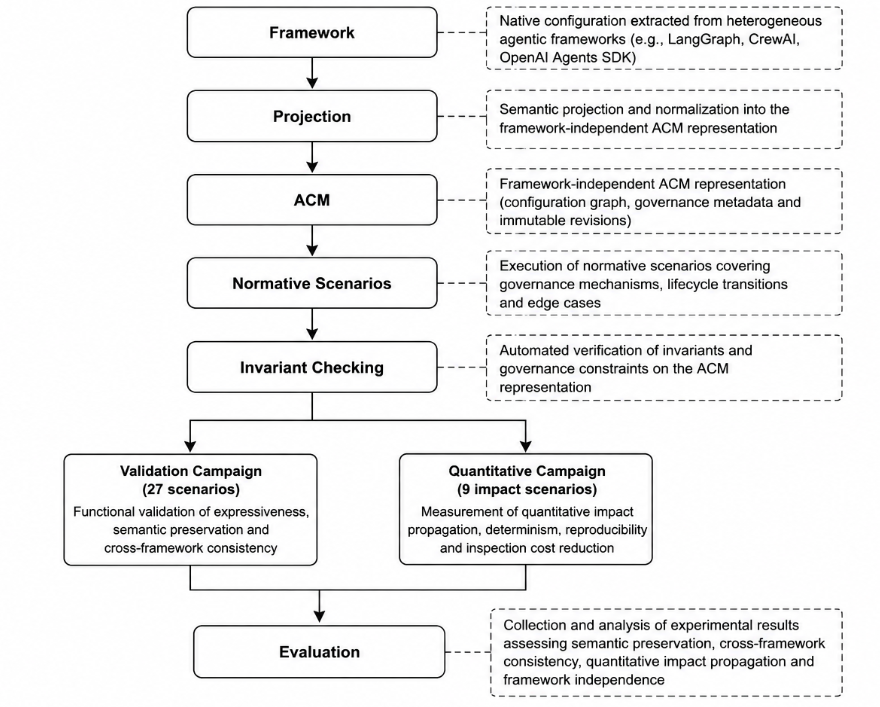
\includegraphics[width=0.5\textwidth]{figures/experimental_protocol.png}
	\caption{Overview of the experimental methodology. Native framework configurations are projected into the ACM reference model through semantic projection, validated using normative governance scenarios and automated invariant checking, and finally evaluated.}
	\label{fig:experimental_protocol}
\end{figure*}

\subsection{Reference Architecture}
\label{subsec:reference_architecture}

The ACM reference model is intentionally independent of any particular agentic framework. Its operationalization therefore adopts a layered architecture that cleanly separates framework-specific extraction from framework-independent governance. This separation preserves the conceptual independence of the reference model while allowing heterogeneous agentic systems to be represented through a common governed configuration.

In our reference architecture, framework-specific adapters extract native constructs and project them into canonical ACM revisions and relationships. All subsequent validation, propagation, assurance, eligibility, and runtime reconstruction operate exclusively on the resulting ACM representation.

The governance kernel constitutes the core of the operationalization. It implements the normative semantics introduced in Section~\ref{sec:governance_semantics}, including structural validation, lifecycle management, governance state evaluation, impact propagation, assurance evaluation, and eligibility assessment. Since these operations manipulate only canonical ACM representations, their behavior remains independent of the execution framework.

The runtime interface complements the governance kernel by exposing governed configurations together with normalized execution observations. Runtime events enrich the operational view of the system without modifying immutable configuration revisions, thereby preserving the separation between configuration governance and execution behavior.

The reference implementation should not be interpreted as a production platform or a preferred execution environment. Its purpose is to demonstrate that the ACM reference model can be operationalized through a framework-independent governance kernel while allowing multiple execution frameworks to share identical governance semantics.

The operationalization is organized into five successive stages:

\begin{enumerate}
	\item \textbf{Framework Extraction}, which retrieves governance-relevant native configuration artifacts exposed by the execution framework;
	
	\item \textbf{Semantic Projection}, which maps these native artifacts onto ACM concepts through framework-specific projection rules;
	
	\item \textbf{Canonical Normalization}, which constructs immutable ACI revisions, resolves references, assigns stable identities, computes canonical digests, and builds the governed configuration graph;
	
	\item \textbf{Governance Processing}, which applies the framework-independent governance semantics defined in Section~\ref{sec:governance_semantics};
	
	\item \textbf{Governed Representation}, which produces the normalized ACM representation used for validation, auditing, replay, impact analysis, and lifecycle management.
\end{enumerate}

This organization deliberately isolates framework-dependent concerns from governance semantics. Native frameworks remain responsible for execution, whereas ACM provides a common governance layer operating on a unified configuration representation.


\subsection{Projection Pipeline}
\label{subsec:semantic_projection_pipeline}

The reference architecture introduced in Section~\ref{subsec:reference_architecture} is realized through a semantic projection pipeline that transforms heterogeneous framework configurations into the canonical ACM representation. Rather than reproducing the internal execution model of each framework, the pipeline identifies only the constructs carrying governance significance and projects them onto the concepts defined by the ACM reference model.

The projection process consists of four successive stages:

\begin{enumerate}
	\item native structure extraction;
	\item semantic classification;
	\item canonical normalization;
	\item projection validation and coverage assessment.
\end{enumerate}

This pipeline establishes a common projection contract shared by all framework adapters. Although extraction mechanisms differ across execution frameworks, each adapter ultimately produces the same normalized ACM representation, enabling the governance kernel to operate independently of framework-specific implementation details.

The complete projection formalism is provided in Appendix~\ref{appendix:projection_formalism}.

\subsubsection{Framework-specific Instantiations}

The prototype implements this projection contract through dedicated adapters for LangGraph, CrewAI, and the OpenAI Agents SDK. These adapters differ only in the extraction phase, reflecting the distinct introspection mechanisms provided by each framework, while sharing the same normalization rules and governance semantics.

For each adapter, the evaluation reports:

\begin{itemize}
	\item the number of governance-relevant native entities;
	\item the number of completely, partially, and unsuccessfully projected entities;
	\item the number of governance-relevant native relationships;
	\item the corresponding entity, relationship, aggregate, and strict coverage scores.
\end{itemize}

The measured values are reported in Section~\ref{sec:evaluation}. They are computed from the explicit inventory of governance-relevant native constructs defined by the experimental protocol rather than inferred from the mere existence of a functioning adapter. Consequently, projection coverage evaluates the expressiveness of the ACM reference model independently of the implementation itself.


\subsection{Framework Adapters}
\label{sec:framework_adapters}

The semantic projection pipeline is realized through framework-specific adapters responsible for extracting governance-relevant configuration artifacts from native execution environments. Although the extraction mechanisms differ across frameworks, every adapter produces the same normalized ACM representation before governance processing begins. Consequently, all subsequent validation, propagation, replay, and lifecycle evaluation operate independently of the originating framework.

The current reference implementation includes adapters for LangGraph, CrewAI, and the OpenAI Agents SDK. These three frameworks intentionally represent complementary introspection regimes rather than alternative implementations of the same architecture, providing a broader validation of the projection approach.

\paragraph{LangGraph.}

LangGraph exposes an explicit execution graph whose nodes, edges, routing conditions, prompts, tools, and models can be extracted directly through framework introspection. Consequently, the projection is predominantly structural and requires only limited semantic reconstruction. Governance-relevant relationships are preserved almost directly before canonical normalization.

\paragraph{CrewAI.}

CrewAI organizes execution around crews, tasks, flows, and associated metadata. While the primary governance entities remain directly identifiable, part of the execution topology must be reconstructed from declarative configuration metadata and execution conventions. The adapter therefore combines explicit extraction with semantic reconstruction while preserving the governance semantics required by ACM.

\paragraph{OpenAI Agents SDK.}

The OpenAI Agents SDK represents agent interactions through explicit handoff relationships. Unlike workflow-oriented frameworks, delegation topology is reconstructed by introspecting agent definitions and their declared handoffs rather than by traversing an explicit workflow graph. This demonstrates that ACM does not depend on a single representation of execution topology and can normalize heterogeneous delegation mechanisms into the same governance model.

Table~\ref{tab:framework_projection_summary} summarizes the principal characteristics of the three adapters.

\begin{table}[t]
	\centering
	\caption{Comparison of framework-specific projection mechanisms.}
	\label{tab:framework_projection_summary}
	\small
	\begin{tabular}{p{3.0cm}p{2.6cm}p{2.8cm}p{2.8cm}}
		\toprule
		\textbf{Characteristic} &
		\textbf{LangGraph} &
		\textbf{CrewAI} &
		\textbf{OpenAI Agents SDK} \\
		\midrule
		Primary topology &
		Explicit execution graph &
		Flow and task structure &
		Agent handoffs \\
		Governance entities &
		Direct extraction &
		Direct extraction &
		Direct extraction \\
		Relationship recovery &
		Structural &
		Hybrid reconstruction &
		Delegation introspection \\
		Semantic normalization &
		Direct &
		Hybrid &
		Direct \\
		Governance kernel &
		Common ACM representation &
		Common ACM representation &
		Common ACM representation \\
		\bottomrule
	\end{tabular}
\end{table}

Together, these adapters cover three complementary introspection regimes while preserving a common governance representation. The objective of the adapters is therefore not to reproduce framework-specific execution semantics but to expose a normalized configuration model suitable for framework-independent governance.
These three adapters demonstrate that the operationalization is not tied to a particular representation of agentic systems. Instead, heterogeneous native abstractions are normalized into a common governance representation that is subsequently processed by the same framework-independent governance algorithms.

\subsection{Governance Algorithms}
\label{sec:governance_algorithms}

The reference implementation realizes the ACM governance semantics through four framework-independent algorithms operating exclusively on normalized ACM representations. Their purpose is not to redefine the formal semantics introduced in Section~\ref{sec:governance_semantics}, but to provide a deterministic operational realization suitable for heterogeneous execution frameworks. Figure~\ref{fig:governance_processing_pipeline} summarizes this workflow.

\begin{figure}[ht]
	\centering
	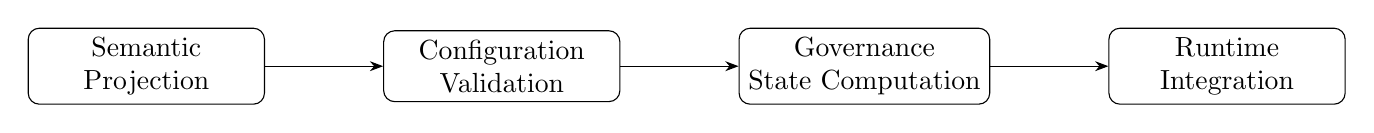
\begin{tikzpicture}[
		node distance=1.5cm,
		every node/.style={
			draw,
			rounded corners,
			align=center,
			minimum width=3cm,
			minimum height=0.8cm
		},
		>=Stealth
		]
		
		\node (projection) {Semantic\\Projection};
		\node (validation) [right=of projection] {Configuration\\Validation};
		\node (states) [right=of validation] {Governance\\State Computation};
		\node (runtime) [right=of states] {Runtime\\Integration};
		
		\draw[->] (projection) -- (validation);
		\draw[->] (validation) -- (states);
		\draw[->] (states) -- (runtime);
		
	\end{tikzpicture}
	
	\caption{Governance processing pipeline implemented by the reference operationalization.}
	\label{fig:governance_processing_pipeline}
\end{figure}

\paragraph{Algorithm 1 --- Semantic Projection}

The projection algorithm transforms native framework artifacts into immutable
ACM revisions and relationships while preserving governance-relevant semantics.

\begin{algorithm}[t]
	\caption{Semantic Projection}
	\begin{enumerate}
		\item \textbf{Input:} native framework configuration.
		\item Extract governance-relevant native entities.
		\item Identify relationships and associated metadata.
		\item Map native constructs to ACM concepts.
		\item Normalize identities and references.
		\item Compute canonical digests.
		\item Construct immutable ACM revisions and relationships.
		\item \textbf{Output:} normalized ACM Configuration Graph.
	\end{enumerate}
\end{algorithm}

\paragraph{Algorithm 2 --- Configuration Validation}

Structural validation verifies the integrity of the normalized configuration
before governance evaluation.

\begin{algorithm}[t]
	\caption{Configuration Validation}
	\begin{enumerate}
		\item \textbf{Input:} normalized ACM Configuration Graph.
		\item Verify structural consistency.
		\item Resolve cross-references.
		\item Validate lifecycle constraints.
		\item Check applicable governance invariants.
		\item Record validation results.
		\item \textbf{Output:} validated Configuration Graph.
	\end{enumerate}
\end{algorithm}

\paragraph{Algorithm 3 --- Governance Evaluation}

Governance evaluation combines local state computation with deterministic
impact propagation until stabilization. The algorithm operationalizes the
semantics defined in Section~\ref{sec:governance_semantics} without redefining
their formal specification.

\begin{algorithm}[t]
	\caption{Governance Evaluation}
	\begin{enumerate}
		\item \textbf{Input:} validated Configuration Graph.
		\item Compute local governance states.
		\item Initialize the impact state from the detected configuration change.
		\item Initialize the propagation worklist.
		\item While the worklist is not empty:
		\begin{enumerate}
			\item select one pending ACI;
			\item propagate impact through applicable relationships;
			\item update impacted dependents when their state increases;
			\item enqueue dependents whose state has changed.
		\end{enumerate}
		\item Evaluate eligibility from the stabilized local and impact states.
		\item \textbf{Output:} governed Configuration Graph.
	\end{enumerate}
\end{algorithm}

\paragraph{Algorithm 4 --- Runtime Integration}

Runtime observations are normalized into governance events that incrementally
reconstruct the Runtime Graph without modifying immutable configuration
revisions.

\begin{algorithm}[t]
	\caption{Runtime Integration}
	\begin{enumerate}
		\item \textbf{Input:} normalized runtime event stream.
		\item For each event:
		\begin{enumerate}
			\item validate event consistency;
			\item append the event to the ordered event log;
			\item apply the event to the current Runtime Graph.
		\end{enumerate}
		\item Replay the ordered event log when reconstruction is requested.
		\item \textbf{Output:} updated or reconstructed Runtime Graph.
	\end{enumerate}
\end{algorithm}

Table~\ref{tab:algorithm_complexity} summarizes the asymptotic complexity of the principal operational algorithms.

\begin{table}[t]
	\centering
	\caption{Asymptotic complexity of the reference algorithms.}
	\label{tab:algorithm_complexity}
	\small
	\begin{tabular}{lc}
		\toprule
		\textbf{Algorithm} & \textbf{Complexity} \\
		\midrule
		Semantic Projection & $O(|V|+|E|)$ \\
		Configuration Validation & $O(|V|+|E|)$ \\
		Governance Evaluation & $O(k(|V|+|E|))$ \\
		Runtime Replay & $O(|R|)$ \\
		\bottomrule
	\end{tabular}
\end{table}

The reference implementation emphasizes deterministic behavior and semantic reproducibility rather than execution performance. The detailed implementation architecture is presented in the following subsection, while the formal properties of the propagation algorithm are established in Section~\ref{sec:governance_semantics} and its appendix.

\subsection{Reference Implementation}
\label{sec:reference_implementation}

The reference implementation provides an executable operationalization of the ACM reference model. It is intended to demonstrate the feasibility and reproducibility of the proposed governance semantics rather than to serve as a production-ready orchestration platform.

The prototype is implemented in Python~3.11--3.13 using Pydantic~v2 to enforce strict data contracts, immutable configuration revisions, and schema validation. Its modular organization separates framework-specific extraction from framework-independent governance, allowing new execution frameworks to be integrated by implementing only an additional projection adapter while leaving the governance kernel unchanged.

The implementation is organized into five principal modules:

\begin{itemize}
	\item \textbf{Core models}, providing immutable ACI revisions, configuration graphs, release baselines, governance descriptors, runtime objects, and canonical serialization;
	\item \textbf{Governance engine}, implementing validation, governance state evaluation, impact propagation, lifecycle management, and runtime reconstruction;
	\item \textbf{Framework adapters}, responsible for semantic projection from native framework representations into canonical ACM objects;
	\item \textbf{Scenario harness}, providing reproducible experimental scenarios, semantic-preservation analyses, quantitative impact evaluation, and report generation;
	\item \textbf{Verification suite}, comprising unit tests, property-based tests, and regression tests validating both the governance semantics and framework projections.
\end{itemize}

Canonical serialization, immutable revisions, and deterministic governance evaluation ensure that identical configurations always produce identical governed representations. This reproducibility is further reinforced by normalized runtime events, replayable execution histories, and deterministic impact propagation, allowing governance analyses to be reproduced independently of the underlying execution framework.

The modular organization also facilitates extensibility. Supporting an additional framework requires only the implementation of a new semantic projection adapter satisfying the common projection contract introduced in Section~\ref{subsec:semantic_projection_pipeline}; the governance kernel, runtime semantics, and evaluation algorithms remain unchanged (see Figure ~\ref{fig:operationalization_acm}).

\begin{figure*}[t]
	\centering
	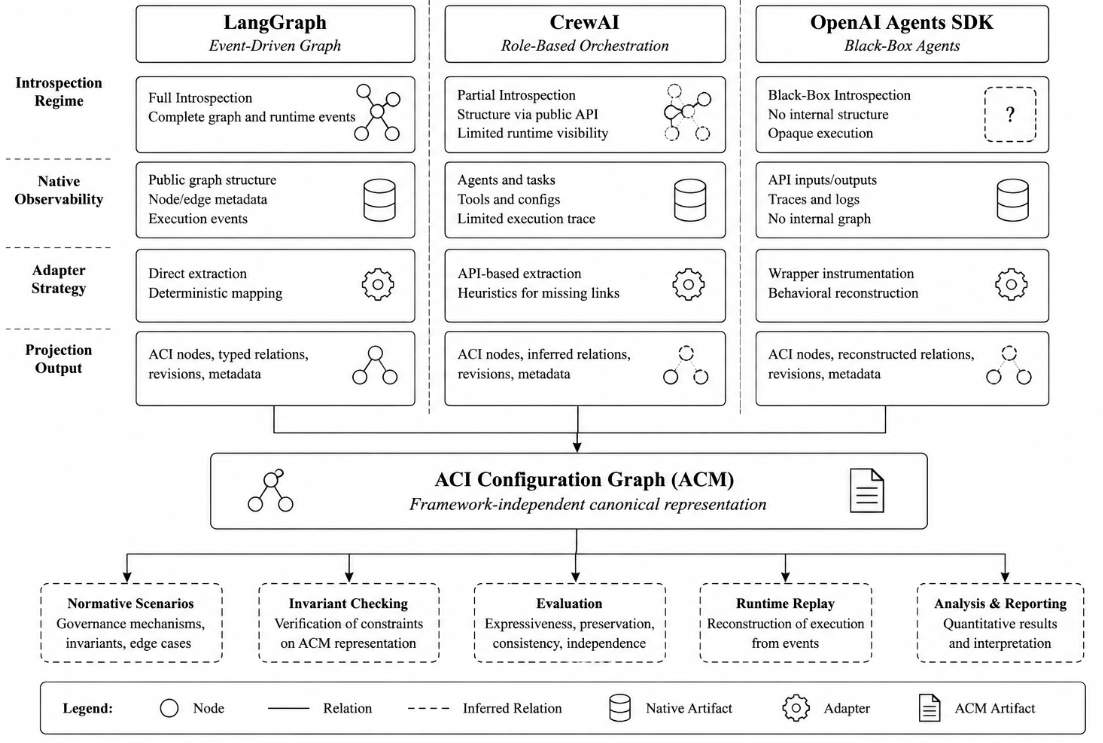
\includegraphics[width=\textwidth]{figures/operationalization_acm.png}
	\caption{Operationalization of the ACM reference model through semantic projection. Native framework configurations are projected into a common framework-independent governance representation, while a reference implementation demonstrates validation, runtime replay and conformance, and impact analysis based on the ACM governance semantics.}
	\label{fig:operationalization_acm}
\end{figure*}
\paragraph{Algorithm Overview}
Table ~\ref{tab:governance_algorithms} summarizes the governance of the implemented algorithms by the ACM reference prototype.

\begin{table}[t]
	\centering
	\caption{Core governance algorithms implemented by the ACM reference prototype.}
	\label{tab:governance_algorithms}
	\small
	\renewcommand{\arraystretch}{1.15}
	\begin{tabularx}{\columnwidth}{>{\raggedright\arraybackslash}p{2.8cm}XX>{\raggedright\arraybackslash}p{2.6cm}}
		\toprule
		\textbf{Algorithm} &
		\textbf{Input} &
		\textbf{Output} &
		\textbf{Main Purpose} \\
		\midrule
		
		Semantic Projection &
		Native framework configuration &
		Canonical ACM configuration graph &
		Semantic normalization \\
		
		Structural Validation &
		ACM configuration graph &
		Validated ACM configuration graph &
		Structural integrity verification \\
		
		Governance Evaluation &
		Validated ACM configuration graph &
		Governance-annotated ACM graph &
		Governance state computation \\
		
		Runtime Integration &
		Normalized runtime events &
		ACM runtime graph &
		Replay and execution reconstruction \\
		
		\bottomrule
	\end{tabularx}
\end{table}

\paragraph{Experimental Instrumentation.}

The reference implementation additionally includes an experimental instrumentation layer used exclusively for the evaluation reported in Section~\ref{sec:evaluation}. This layer collects projection inventories, semantic-preservation outcomes, normalized impact-propagation results, reproducibility metadata, and comparison data used by the experimental protocol. It remains separated from the governance kernel and does not participate in the computation of normative ACM states. This separation ensures that the evaluation infrastructure observes and measures the operationalization without altering the semantics being evaluated.


\section{Evaluation}
\label{sec:evaluation}

This section evaluates the ACM reference model with respect to the research questions introduced in Section~\ref{sec:introduction}. The objective is to assess whether the proposed reference model preserves governance semantics across heterogeneous agentic frameworks, supports deterministic governance evaluation, and provides a framework-independent foundation for agentic configuration management. The evaluation combines two complementary experimental campaigns. The first validates the expressiveness of the reference model, the preservation of its governance semantics, and its cross-framework applicability through twenty-seven governance scenarios executed on LangGraph, CrewAI, and the OpenAI Agents SDK. The second complements this validation with a dedicated quantitative evaluation of impact propagation across nine additional cases. Together, both campaigns provide evidence for the four research questions addressed in this work.

\subsection{Research Questions}
\label{sec:research_questions}

The evaluation addresses the following research questions.

\begin{itemize}
	
	\item \textbf{RQ1 -- Reference Model Expressiveness.}
	Can heterogeneous agentic frameworks be represented using the ACM reference model while preserving governance-relevant configuration concepts?
	
	\item \textbf{RQ2 -- Governance Semantics.}
	Does the operationalization faithfully realize the governance semantics defined in Section~\ref{sec:governance_semantics}, including lifecycle management, governance evaluation, impact propagation, release governance, and runtime reconstruction?
	
	\item \textbf{RQ3 -- Framework Independence.}
	Can equivalent governed representations be obtained from heterogeneous execution frameworks through semantic projection into a common ACM representation?
	
	\item \textbf{RQ4 -- Quantitative Impact Analysis.}
	Can the governance kernel produce deterministic and reproducible impact analyses across heterogeneous frameworks while reducing the set of configuration elements requiring manual inspection?
	
\end{itemize}

The first three research questions evaluate the reference model itself, whereas the fourth assesses the operational behavior of the governance kernel through a dedicated quantitative impact analysis.
The following sections describe the experimental methodology adopted to answer these research questions and present the empirical evidence collected using the reference implementation.


\subsection{Experimental Design}
\label{sec:experimental_protocol}

The evaluation follows two complementary experimental campaigns designed to assess distinct properties of the ACM reference model.

\subsubsection{Campaign A -- Reference Model Validation} The first campaign evaluates the expressiveness of the reference model, the preservation of its governance semantics, and its applicability across heterogeneous agentic frameworks. It consists of twenty-seven controlled governance scenarios covering the principal concepts introduced throughout the reference model, including immutable revisions, lifecycle evolution, governance states, dependency propagation, release baselines, runtime governance, dynamic agents, and semantic projection. The complete scenario suite is executed independently on LangGraph, CrewAI, and the OpenAI Agents SDK through their respective projection adapters. Each native configuration is projected into the canonical ACM representation before governance processing, while the same framework-independent governance kernel is used for all three frameworks. This design makes it possible to distinguish framework-specific extraction from the semantics evaluated by the ACM core. Each scenario specifies an initial governed configuration, the sequence of configuration or runtime events applied to the system, and the expected governance outcomes. The resulting governed representations are compared against the expected semantic properties defined by the reference model. Collectively, the twenty-seven scenarios provide evidence for RQ1 and RQ2, while their execution across the three frameworks directly supports RQ3 by testing whether heterogeneous native representations converge toward equivalent governed ACM representations (Table ~\ref{tab:qualitative_validation} summarizes the main results associated to the Research Questions). 

\begin{table}[t]
	\caption{Coverage of the qualitative validation campaign. The 27 governance scenarios collectively exercise the main semantic capabilities of the ACM reference model across the supported execution frameworks.}
	\label{tab:qualitative_validation}
	\centering
	\footnotesize
	\begin{tabular}{p{3.2cm}p{4.5cm}p{1.8cm}c}
		\toprule
		\textbf{Validation aspect} &
		\textbf{Representative capabilities} &
		\textbf{Research question(s)} &
		\textbf{Result} \\
		\midrule
		
		Configuration model
		&
		ACI revisions, configuration relationships, release baselines, governance descriptors
		&
		RQ1
		&
		Passed
		\\
		
		Governance semantics
		&
		Lifecycle transitions, quality assessment, assurance evaluation, impact propagation, eligibility computation
		&
		RQ2
		&
		Passed
		\\
		
		Framework-independent projection
		&
		Semantic projection from LangGraph, CrewAI, and OpenAI Agents SDK into a common ACM representation
		&
		RQ3
		&
		Passed
		\\
		
		Runtime governance
		&
		Runtime event representation, execution replay, provenance reconstruction, deterministic state reconstruction
		&
		RQ2, RQ3
		&
		Passed
		\\
		
		Cross-framework consistency
		&
		Equivalent governance outcomes obtained from semantically equivalent native implementations
		&
		RQ3
		&
		Passed
		\\
		
		\bottomrule
	\end{tabular}
\end{table}

\subsubsection{Campaign B -- Quantitative Impact Evaluation} The second campaign focuses specifically on the quantitative behavior of impact propagation. Three representative configuration changes are evaluated for each of the same three frameworks, corresponding to local, intermediate, and global propagation scopes, resulting in nine additional experimental cases. Each case is executed five consecutive times to assess deterministic behavior and reproducibility. The same framework-independent fixed-point propagation engine is used throughout the evaluation. For every experimental case, the evaluation records the governed impact set, impact size, impact ratio, comparison with pre-specified reference impact sets established independently from the propagation engine, fixed-point convergence characteristics, reproducibility indicators, and estimated inspection reduction. This second campaign provides dedicated quantitative evidence for RQ4 while complementing the broader semantic validation performed in Campaign A  (see Figure ~\ref{fig:evaluation_methodology} that summarizes the methodology). 

\begin{figure}[ht]
	\centering
	
	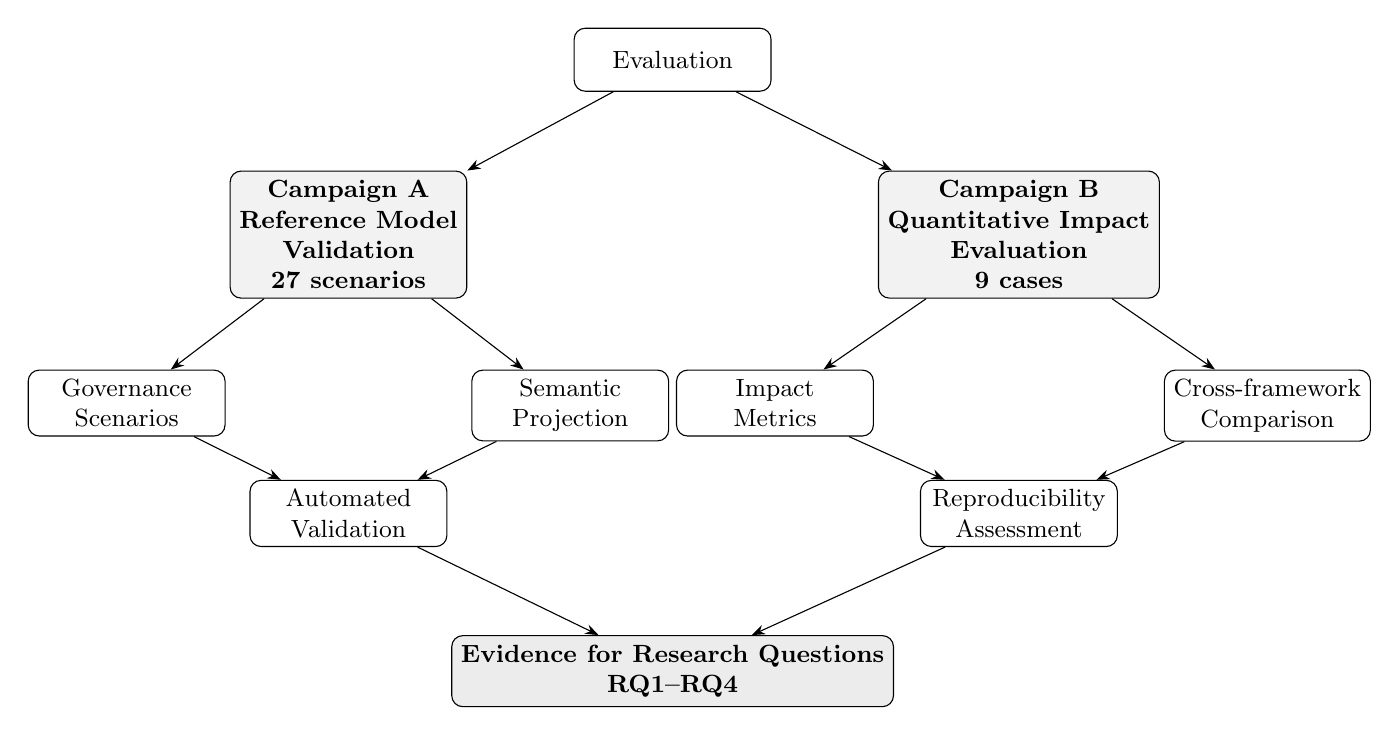
\begin{tikzpicture}[
		node distance=0.8cm and 1cm,
		>=Stealth,
		process/.style={
			draw,
			rounded corners,
			align=center,
			minimum width=2.5cm,
			minimum height=0.8cm,
			font=\small
		},
		campaign/.style={
			draw,
			rounded corners,
			fill=gray!10,
			align=center,
			minimum width=3cm,
			minimum height=0.8cm,
			font=\small\bfseries
		},
		rq/.style={
			draw,
			rounded corners,
			fill=gray!15,
			align=center,
			minimum width=3.8cm,
			minimum height=0.7cm,
			font=\small\bfseries
		}
		]
		
		% Top
		\node[process] (eval) {Evaluation};
		
		% Campaigns
		\node[campaign, below left=1cm and 1.35cm of eval] (campA)
		{Campaign A\\Reference Model\\Validation\\27 scenarios};
		
		\node[campaign, below right=1cm and 1.35cm of eval] (campB)
		{Campaign B\\Quantitative Impact\\Evaluation\\9 cases};
		
		% Campaign A activities
		\node[process, below left=0.9cm and 0.05cm of campA] (scenarios)
		{Governance\\Scenarios};
		
		\node[process, below right=0.9cm and 0.05cm of campA] (projection)
		{Semantic\\Projection};
		
		% Campaign B activities
		\node[process, below left=0.9cm and 0.05cm of campB] (impact)
		{Impact\\Metrics};
		
		\node[process, below right=0.9cm and 0.05cm of campB] (comparison)
		{Cross-framework\\Comparison};
		
		% Intermediate evidence nodes
		\node[process, below=2.3cm of campA] (validation)
		{Automated\\Validation};
		
		\node[process, below=2.3cm of campB] (repro)
		{Reproducibility\\Assessment};
		
		% Bottom
		\node[rq, below=1.5cm of eval, yshift=-5.4cm] (rqs)
		{Evidence for Research Questions\\RQ1--RQ4};
		
		% Connections
		\draw[->] (eval) -- (campA);
		\draw[->] (eval) -- (campB);
		
		\draw[->] (campA) -- (scenarios);
		\draw[->] (campA) -- (projection);
		\draw[->] (scenarios) -- (validation);
		\draw[->] (projection) -- (validation);
		
		\draw[->] (campB) -- (impact);
		\draw[->] (campB) -- (comparison);
		\draw[->] (impact) -- (repro);
		\draw[->] (comparison) -- (repro);
		
		\draw[->] (validation) -- (rqs);
		\draw[->] (repro) -- (rqs);
		
	\end{tikzpicture}
	
	\caption{Experimental methodology adopted to evaluate the ACM reference model. Campaign A validates the reference model through 27 governance scenarios and semantic projection, whereas Campaign B evaluates quantitative impact propagation across nine cross-framework cases. Together, both campaigns provide complementary evidence for RQ1--RQ4.}
	
	\label{fig:evaluation_methodology}
	
\end{figure}

Table~\ref{tab:rq_validation} summarizes how the two complementary experimental campaigns collectively address the four research questions investigated in this work.
\begin{table}[t]
	\caption{Relationship between the research questions, the experimental evidence, and the corresponding validation results.}
	\label{tab:rq_validation}
	\centering
	\footnotesize
	\begin{tabular}{p{1.0cm}p{4.0cm}p{4.2cm}p{3.0cm}}
		\toprule
		\textbf{RQ} &
		\textbf{Research objective} &
		\textbf{Experimental evidence} &
		\textbf{Main result} \\
		\midrule
		
		RQ1 &
		Can ACM represent heterogeneous agentic configurations using a unified governance model?
		&
		Qualitative validation campaign (27 governance scenarios) covering the complete ACM metamodel.
		&
		All evaluated configuration concepts were successfully represented using the ACM reference model.
		\\
		
		RQ2 &
		Does ACM preserve governance semantics independently of the native execution framework?
		&
		Cross-framework execution of governance scenarios, including lifecycle, quality, assurance, impact propagation, runtime reconstruction, and baseline evaluation.
		&
		Equivalent governance semantics were obtained after semantic projection across all evaluated frameworks.
		\\
		
		RQ3 &
		Can ACM provide a framework-independent governance layer?
		&
		Semantic projection of LangGraph, CrewAI, and OpenAI Agents SDK into a common ACM representation.
		&
		Framework-specific implementations produced equivalent governed configuration graphs and governance outcomes.
		\\
		
		RQ4 &
		Can ACM quantitatively characterize configuration impact while remaining deterministic and reproducible?
		&
		Quantitative impact evaluation on nine representative change scenarios executed across three frameworks with repeated executions.
		&
		Deterministic impact propagation, identical governed impact sets across frameworks, and reproducible quantitative metrics were obtained for all evaluated scenarios.
		\\
		
		\bottomrule
	\end{tabular}
\end{table}

\subsection{Validation of the Reference Model}
\label{sec:reference_model_validation}

Campaign~A evaluates the ACM reference model through a suite of twenty-seven controlled governance scenarios executed independently on LangGraph, CrewAI, and the OpenAI Agents SDK. The objective is not to benchmark execution performance, but to verify that heterogeneous native configurations can be projected into equivalent governed ACM representations while preserving the governance semantics defined in Section~\ref{sec:governance_semantics}.

The scenario suite was designed to exercise the principal concepts introduced throughout the reference model. Collectively, the scenarios cover immutable ACI revisions, lifecycle evolution, governance states, structural relationships, semantic projection, release baselines, runtime governance, dependency propagation, and dynamic agent evolution. Rather than validating isolated software components, each scenario evaluates the interaction between several governance mechanisms under representative configuration changes.

For every scenario, equivalent native configurations were implemented for the three supported frameworks. After semantic projection, the resulting ACM representations were processed by the same framework-independent governance kernel. The observed governed representations were then compared against the expected governance outcomes defined by the experimental specification. This protocol evaluates both the correctness of semantic projection and the preservation of governance semantics independently of the originating execution framework.

Table~\ref{tab:scenario_categories} summarizes the categories covered by the experimental campaign.

\begin{table}[t]
	\centering
	\caption{Coverage of the reference model validation scenarios.}
	\label{tab:scenario_categories}
	\small
	\begin{tabular}{p{3.2cm}p{3.8cm}}
		\toprule
		\textbf{Category} & \textbf{Representative governance aspects} \\
		\midrule
		Revision management &
		Immutable revisions, promotion, lifecycle evolution \\
		Dependency management &
		Structural relationships and impact dependencies \\
		Governance evaluation &
		Eligibility assessment, governance states, policy evaluation \\
		Release governance &
		Baseline composition, revision consistency, release evolution \\
		Runtime governance &
		Execution events and runtime reconstruction \\
		Dynamic evolution &
		Dynamic agents and evolving configurations \\
		Semantic projection &
		Cross-framework normalization and representation consistency \\
		\bottomrule
	\end{tabular}
\end{table}

Across the complete campaign, the twenty-seven scenarios produced governed representations consistent with the expected semantic properties on all three execution frameworks. No framework-specific governance behavior was introduced after semantic projection, indicating that governance evaluation depends exclusively on the normalized ACM representation rather than on the native execution model.

These observations provide complementary evidence for the first three research questions. The breadth of the scenario suite supports the expressiveness of the reference model (RQ1), the agreement between the operationalization and the formal governance semantics (RQ2), and the ability to obtain equivalent governed representations from heterogeneous execution frameworks through semantic projection (RQ3). The quantitative characteristics of impact propagation are evaluated separately in Campaign~B.

\subsection{Cross-framework Semantic Projection}
\label{sec:cross_framework_projection}

The objective of this evaluation is to determine whether heterogeneous execution frameworks can be projected into equivalent governed ACM representations while preserving the governance-relevant information required by the reference model. This experiment addresses RQ3 by evaluating the semantic projection implemented for LangGraph, CrewAI, and the OpenAI Agents SDK.

Although the three frameworks support comparable agentic applications, they expose substantially different introspection mechanisms. LangGraph provides an explicit workflow graph whose nodes and structural relationships can be reconstructed directly through framework introspection. CrewAI separates orchestration into Crew and Flow abstractions, requiring part of the execution topology to be reconstructed from adapter metadata because the complete graph is not statically introspectable. In contrast, the OpenAI Agents SDK exposes delegation explicitly through agent handoffs, allowing the delegation graph to be reconstructed directly while agent-level references remain normalized through adapter metadata. These three frameworks therefore represent complementary introspection regimes while sharing the same ACM governance model after semantic projection.

To evaluate information preservation, representative native workflows were extracted independently from each framework and compared with manually established golden representations over the normative ACM perimeter. Each extracted property was classified as \emph{preserved}, \emph{approximated}, or \emph{unsupported}, allowing the evaluation to distinguish exact reconstruction from intentional semantic abstraction.

Table~\ref{tab:projection_results} summarizes the principal information-preservation metrics obtained across the three frameworks.

\begin{table*}[t]
	\centering
	\caption{Summary of information preservation after semantic projection.}
	\label{tab:projection_results}
	\small
	\begin{tabular}{lccc}
		\toprule
		\textbf{Metric}
		&
		\textbf{LangGraph}
		&
		\textbf{CrewAI}
		&
		\textbf{OpenAI Agents SDK}
		\\
		\midrule
		Node coverage & 100\% & 100\% & 100\% \\
		Relationship coverage & 100\% & 100\% & 100\% \\
		Branch coverage & 100\% & 100\% & 100\% \\
		Entry point preserved & Yes & Yes & Yes \\
		Terminal nodes preserved & Yes & Yes & Yes \\
		Agent--prompt references & 100\% & 100\% & 100\% \\
		Agent--tool references & 100\% & 100\% & 100\% \\
		Stable extraction digest & Yes & Yes & Yes \\
		Normative properties preserved & 10 & 9--10 & 10 \\
		Approximated properties & 1 & 1 & 1 \\
		Unsupported properties & 0 & 0--1 & 0 \\
		\bottomrule
	\end{tabular}
\end{table*}

While the overall preservation results are comparable, the extraction process differs significantly between frameworks. LangGraph exposes its execution topology directly through the native workflow graph. CrewAI illustrates the limits of static introspection: workflow nodes are extracted from the Flow definition, whereas part of the orchestration topology must be supplied through adapter metadata because it is resolved dynamically at execution time. Conversely, the OpenAI Agents SDK exposes the delegation topology explicitly through handoff relationships, allowing the corresponding graph to be reconstructed entirely by introspection without unresolved structural elements.

These observations demonstrate that ACM does not depend on a single execution abstraction or introspection mechanism. Instead, semantic projection normalizes heterogeneous native representations into a common governed configuration while explicitly documenting the origin of extracted information. Consequently, differences in framework introspectability remain confined to the extraction stage and do not affect the governance semantics subsequently evaluated by the framework-independent governance kernel.

Collectively, these results support RQ3 by showing that heterogeneous native representations converge toward equivalent ACM governance models despite relying on fundamentally different extraction mechanisms. The quantitative behavior of the resulting governance semantics is evaluated separately in Campaign~B.

\subsection{Research Questions}
\label{sec:research_questions}

The evaluation addresses the following research questions.

\begin{itemize}
	
	\item \textbf{RQ1 -- Reference Model Expressiveness.}
	Can heterogeneous agentic frameworks be represented using the ACM reference model while preserving governance-relevant configuration concepts?
	
	\item \textbf{RQ2 -- Governance Semantics.}
	Does the operationalization faithfully realize the governance semantics defined in Section~\ref{sec:governance_semantics}, including lifecycle management, governance evaluation, impact propagation, release governance, and runtime reconstruction?
	
	\item \textbf{RQ3 -- Framework Independence.}
	Can equivalent governed representations be obtained from heterogeneous execution frameworks through semantic projection into a common ACM representation?
	
	\item \textbf{RQ4 -- Quantitative Impact Analysis.}
	Can the governance kernel produce deterministic and reproducible impact analyses across heterogeneous frameworks while reducing the set of configuration elements requiring manual inspection?
	
\end{itemize}

The first three research questions evaluate the reference model itself, whereas the fourth assesses the operational behavior of the governance kernel through a dedicated quantitative impact analysis.
The following sections describe the experimental methodology adopted to answer these research questions and present the empirical evidence collected using the reference implementation.

Figure ~\ref{fig:introspection_framework} summarizes the overall experimental design.
\begin{figure*}[t]
	\centering
	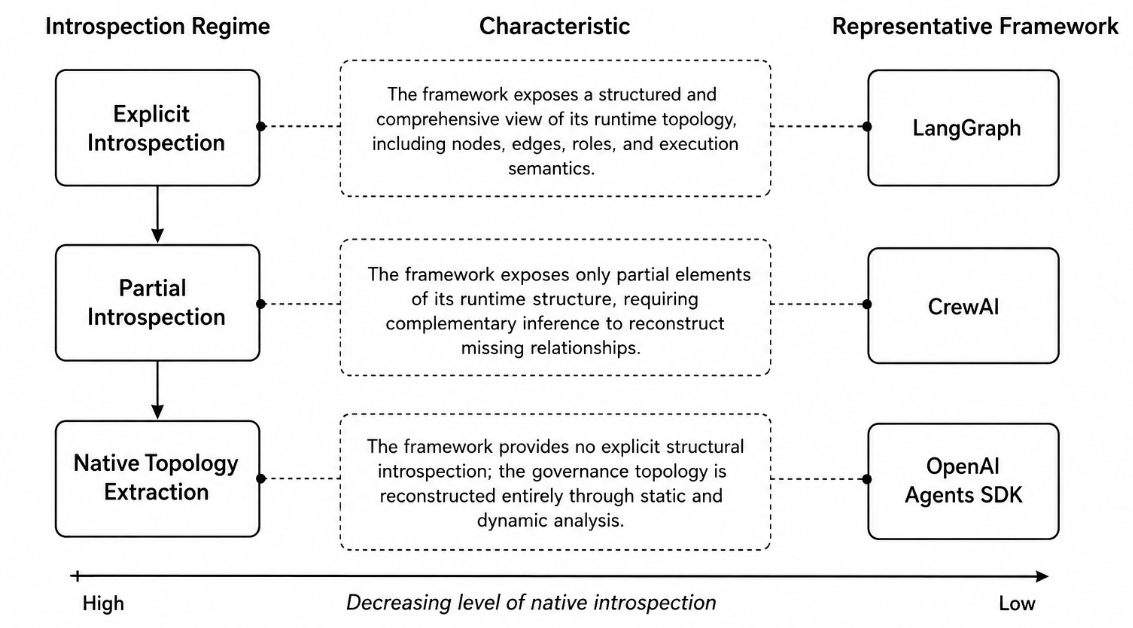
\includegraphics[width=0.7\textwidth]{figures/introspection_framework.png}
	\caption{The three introspection regimes of the evaluated frameworks. From explicit runtime introspection to native topological extraction, ACM relies on semantic projection to reconstruct a unified governance topology across heterogeneous execution platforms}
	\label{fig:introspection_framework}
\end{figure*}

\subsection{Validation of the Reference Model}
\label{sec:reference_model_validation}

Campaign~A evaluates the ACM reference model through a suite of twenty-seven controlled governance scenarios executed independently on LangGraph, CrewAI, and the OpenAI Agents SDK. The objective is not to benchmark execution performance, but to verify that heterogeneous native configurations can be projected into equivalent governed ACM representations while preserving the governance semantics defined in Section~\ref{sec:governance_semantics}.

The scenario suite was designed to exercise the principal concepts introduced throughout the reference model. Collectively, the scenarios cover immutable ACI revisions, lifecycle evolution, governance states, structural relationships, semantic projection, release baselines, runtime governance, dependency propagation, and dynamic agent evolution. Rather than validating isolated software components, each scenario evaluates the interaction between several governance mechanisms under representative configuration changes.

For every scenario, equivalent native configurations were implemented for the three supported frameworks. After semantic projection, the resulting ACM representations were processed by the same framework-independent governance kernel. The observed governed representations were then compared against the expected governance outcomes defined by the experimental specification. This protocol evaluates both the correctness of semantic projection and the preservation of governance semantics independently of the originating execution framework.

Table~\ref{tab:scenario_categories} summarizes the categories covered by the experimental campaign.

\begin{table}[t]
	\centering
	\caption{Coverage of the reference model validation scenarios.}
	\label{tab:scenario_categories}
	\small
	\begin{tabular}{p{3.2cm}p{3.8cm}}
		\toprule
		\textbf{Category} & \textbf{Representative governance aspects} \\
		\midrule
		Revision management &
		Immutable revisions, promotion, lifecycle evolution \\
		Dependency management &
		Structural relationships and impact dependencies \\
		Governance evaluation &
		Eligibility assessment, governance states, policy evaluation \\
		Release governance &
		Baseline composition, revision consistency, release evolution \\
		Runtime governance &
		Execution events and runtime reconstruction \\
		Dynamic evolution &
		Dynamic agents and evolving configurations \\
		Semantic projection &
		Cross-framework normalization and representation consistency \\
		\bottomrule
	\end{tabular}
\end{table}

Across the complete campaign, the twenty-seven scenarios produced governed representations consistent with the expected semantic properties on all three execution frameworks. No framework-specific governance behavior was introduced after semantic projection, indicating that governance evaluation depends exclusively on the normalized ACM representation rather than on the native execution model.

These observations provide complementary evidence for the first three research questions. The breadth of the scenario suite supports the expressiveness of the reference model (RQ1), the agreement between the operationalization and the formal governance semantics (RQ2), and the ability to obtain equivalent governed representations from heterogeneous execution frameworks through semantic projection (RQ3). The quantitative characteristics of impact propagation are evaluated separately in Campaign~B.

\subsection{Cross-framework Semantic Projection}
\label{sec:cross_framework_projection}

The first objective of the experimental evaluation is to determine whether heterogeneous execution frameworks can be projected into equivalent governed ACM representations. This evaluation addresses RQ3 by comparing the semantic projection produced for LangGraph, CrewAI, and the OpenAI Agents SDK over the complete suite of twenty-seven governance scenarios.

Although these frameworks expose different execution abstractions, they represent complementary introspection regimes. LangGraph provides an explicit execution graph, CrewAI combines declarative configuration with runtime metadata, whereas the OpenAI Agents SDK represents coordination primarily through agent definitions and handoff relationships. The semantic projection adapters introduced in Section~\ref{sec:framework_adapters} normalize these heterogeneous representations into the common ACM configuration model before governance evaluation.

For every scenario, the projected ACM representation was evaluated with respect to governance-relevant entities, structural relationships, lifecycle information, and dependency semantics. Projection completeness was measured using the entity, relationship, aggregate, and strict coverage metrics introduced in the experimental protocol.

Table~\ref{tab:projection_results} summarizes the projection results obtained for the three frameworks.

\begin{table}[t]
	\centering
	\caption{Summary of Campaign A validation results.}
	\label{tab:campaign_a_summary}
	\small
	\begin{tabular}{lr}
		\toprule
		\textbf{Metric} & \textbf{Value} \\
		\midrule
		Governance scenarios & 27 \\
		Verification tests executed & 295 \\
		Passed & 24 \\
		Passed with documented deviation & 3 \\
		Failed & 0 \\
		Skipped & 0 \\
		Not executed & 0 \\
		\bottomrule
	\end{tabular}
\end{table}

Across the twenty-seven scenarios, all three adapters successfully produced governed ACM representations compatible with the common governance kernel. Differences remained limited to framework-specific extraction mechanisms and did not affect the normalized governance representation used for subsequent evaluation.

These observations support RQ3 by showing that the operational semantics implemented by ACM are independent of the native execution framework once semantic projection has been completed. The resulting governed representations provide a common basis for lifecycle evaluation, impact propagation, release governance, and runtime reconstruction across heterogeneous agentic ecosystems.

\subsection{Quantitative Impact Evaluation}
\label{sec:quantitative_impact}

Campaign~B complements the qualitative validation performed in the previous sections by evaluating the quantitative behavior of the ACM impact propagation semantics. Whereas Campaign~A verifies that the governance semantics are correctly preserved, Campaign~B measures the properties of the resulting propagation across representative configuration changes.

Nine experimental cases were constructed by combining the three supported execution frameworks with three representative change classes corresponding to local, intermediate, and global propagation scopes. Every experimental case was executed five consecutive times using the same framework-independent governance kernel.

The quantitative evaluation measures five complementary properties:

\begin{itemize}
	\item propagation extent through the impacted set size ($|P_f(c)|$);
	\item normalized propagation ratio with respect to the configuration graph;
	\item agreement with independently derived pre-specified reference impact sets using precision, recall, and F$_1$ score;
	\item reduction of the manual inspection effort;
	\item reproducibility of the fixed-point computation.
\end{itemize}

The reported inspection reduction values represent protocol-level estimates rather than measurements obtained from a controlled user study. They are computed by comparing the number of manual inspections required for an exhaustive native impact analysis with the number of residual inspections required after the governed impact set has been produced by ACM. Consequently, these values should be interpreted as an estimate of the potential reduction in manual verification effort within the experimental protocol. An empirical assessment involving human evaluators remains part of future work.

Table~\ref{tab:impact_summary} summarizes the principal quantitative results.

\begin{table*}[t]
	\centering
	\caption{Summary of the quantitative impact evaluation.}
	\label{tab:impact_summary}
	\small
	\begin{tabular}{llcccccc}
		\toprule
		Framework &
		Change &
		Impact Size &
		Impact Ratio &
		Precision &
		Recall &
		F$_1$ &
		Inspection Reduction
		\\
		\midrule
		LangGraph &
		Local &
		2 &
		0.182 &
		1.00 &
		1.00 &
		1.00 &
		0.846
		\\
		&
		Intermediate &
		2 &
		0.182 &
		1.00 &
		1.00 &
		1.00 &
		0.692
		\\
		&
		Global &
		5 &
		0.455 &
		1.00 &
		1.00 &
		1.00 &
		0.615
		\\
		\midrule
		CrewAI &
		Local &
		2 &
		0.182 &
		1.00 &
		1.00 &
		1.00 &
		0.846
		\\
		&
		Intermediate &
		2 &
		0.182 &
		1.00 &
		1.00 &
		1.00 &
		0.692
		\\
		&
		Global &
		5 &
		0.455 &
		1.00 &
		1.00 &
		1.00 &
		0.615
		\\
		\midrule
		OpenAI Agents &
		Local &
		2 &
		0.182 &
		1.00 &
		1.00 &
		1.00 &
		0.846
		\\
		&
		Intermediate &
		2 &
		0.182 &
		1.00 &
		1.00 &
		1.00 &
		0.692
		\\
		&
		Global &
		5 &
		0.455 &
		1.00 &
		1.00 &
		1.00 &
		0.615
		\\
		\bottomrule
	\end{tabular}
\end{table*}

The impact metrics remained identical across the three execution frameworks for every change class. Local and intermediate changes affected two governed ACIs, whereas global model updates propagated to five governed ACIs. The corresponding impact ratios remained consistent across frameworks, reflecting the identical normalized configuration graph obtained after semantic projection. 

Across all nine experimental cases, the governed impact sets produced by the fixed-point propagation engine exactly matched the pre-specified reference impact sets, yielding precision, recall, and F$_1$ values equal to~1.0 without false positives or false negatives. These reference impact sets were established from the native framework definitions prior to executing the ACM propagation engine and remained external to the governance kernel throughout the evaluation. Consequently, precision, recall, and F$_1$ quantify agreement between the governed impact sets and these pre-specified reference sets rather than accuracy with respect to an independently adjudicated ground truth. The comparison itself is performed through a framework-independent set comparison module, ensuring that the evaluation procedure remains structurally independent of the propagation implementation.

The evaluation also indicates a substantial reduction in the residual manual inspection effort, ranging from 61.5\% for global changes to 84.6\% for local changes under the experimental protocol. These values quantify the reduction in configuration elements requiring human verification after ACM has identified the governed impact set; they do not represent execution-time performance measurements. 

Collectively, these observations provide quantitative evidence supporting RQ4. They indicate that the governance kernel produces deterministic and framework-independent impact analyses while maintaining complete agreement with the pre-specified reference impact sets across the evaluated scenarios. Reproducibility and convergence characteristics are analyzed in the following subsection.

Across the twenty-seven scenarios, all three adapters successfully produced governed ACM representations compatible with the common governance kernel. Differences remained limited to framework-specific extraction mechanisms and did not affect the normalized governance representation used for subsequent evaluation.

These observations support RQ3 by showing that the operational semantics implemented by ACM are independent of the native execution framework once semantic projection has been completed. The resulting governed representations provide a common basis for lifecycle evaluation, impact propagation, release governance, and runtime reconstruction across heterogeneous agentic ecosystems.

\subsection{Quantitative Impact Evaluation}
\label{sec:quantitative_impact}

Campaign~B complements the qualitative validation performed in the previous sections by evaluating the quantitative behavior of the ACM impact propagation semantics. Whereas Campaign~A verifies that the governance semantics are correctly preserved, Campaign~B measures the properties of the resulting propagation across representative configuration changes.

Nine experimental cases were constructed by combining the three supported execution frameworks with three representative change classes corresponding to local, intermediate, and global propagation scopes. Every experimental case was executed five consecutive times using the same framework-independent governance kernel.

The quantitative evaluation measures five complementary properties:

\begin{itemize}
	\item propagation extent through the impacted set size ($|P_f(c)|$);
	\item normalized propagation ratio with respect to the configuration graph;
	\item agreement with independently derived pre-specified reference impact sets using precision, recall, and F$_1$ score;
	\item reduction of the manual inspection effort;
	\item reproducibility of the fixed-point computation.
\end{itemize}

Table~\ref{tab:impact_summary} summarizes the principal quantitative results.

\begin{table*}[t]
	\centering
	\caption{Summary of the quantitative impact evaluation.}
	\label{tab:impact_summary}
	\small
	\begin{tabular}{llcccccc}
		\toprule
		Framework &
		Change &
		Impact Size &
		Impact Ratio &
		Precision &
		Recall &
		F$_1$ &
		Inspection Reduction
		\\
		\midrule
		LangGraph &
		Local &
		2 &
		0.182 &
		1.00 &
		1.00 &
		1.00 &
		0.846
		\\
		&
		Intermediate &
		2 &
		0.182 &
		1.00 &
		1.00 &
		1.00 &
		0.692
		\\
		&
		Global &
		5 &
		0.455 &
		1.00 &
		1.00 &
		1.00 &
		0.615
		\\
		\midrule
		CrewAI &
		Local &
		2 &
		0.182 &
		1.00 &
		1.00 &
		1.00 &
		0.846
		\\
		&
		Intermediate &
		2 &
		0.182 &
		1.00 &
		1.00 &
		1.00 &
		0.692
		\\
		&
		Global &
		5 &
		0.455 &
		1.00 &
		1.00 &
		1.00 &
		0.615
		\\
		\midrule
		OpenAI Agents &
		Local &
		2 &
		0.182 &
		1.00 &
		1.00 &
		1.00 &
		0.846
		\\
		&
		Intermediate &
		2 &
		0.182 &
		1.00 &
		1.00 &
		1.00 &
		0.692
		\\
		&
		Global &
		5 &
		0.455 &
		1.00 &
		1.00 &
		1.00 &
		0.615
		\\
		\bottomrule
	\end{tabular}
\end{table*}

The impact metrics remained identical across the three execution frameworks for every change class. Local and intermediate changes affected two governed ACIs, whereas global model updates propagated to five governed ACIs. The corresponding impact ratios remained consistent across frameworks, reflecting the identical normalized configuration graph obtained after semantic projection. 

Across all nine experimental cases, the governed impact sets produced by the fixed-point propagation engine exactly matched the pre-specified reference impact sets, yielding precision, recall, and F$_1$ values equal to~1.0 without false positives or false negatives. The comparison procedure is intentionally separated from the governance kernel: the reference impact sets constitute external experimental artifacts established independently of the propagation engine and compared through a framework-independent set comparison module. 

The evaluation also indicates a substantial reduction in the residual manual inspection effort, ranging from 61.5\% for global changes to 84.6\% for local changes under the experimental protocol. These values quantify the reduction in configuration elements requiring human verification after ACM has identified the governed impact set; they do not represent execution-time performance measurements. 

Collectively, these observations provide quantitative evidence supporting RQ4. They indicate that the governance kernel produces deterministic and framework-independent impact analyses while maintaining complete agreement with the pre-specified reference impact sets across the evaluated scenarios. Reproducibility and convergence characteristics are analyzed in the following subsection.




\subsection{Reproducibility}
\label{subsec:reproducibility}

Beyond semantic correctness, the evaluation assesses the reproducibility of the proposed governance semantics. All experimental campaigns were executed using the same framework-independent governance kernel, while semantic projection was performed independently for LangGraph, CrewAI, and the OpenAI Agents SDK.

Campaign~A executed the complete suite of twenty-seven governance scenarios on each framework, producing consistent governed ACM representations and identical validation outcomes independently of the originating execution environment. Campaign~B complemented this validation through nine quantitative impact scenarios, each executed five consecutive times. Across all repetitions, the governance kernel produced identical impacted sets, identical governance states, and identical quantitative metrics.

The fixed-point propagation algorithm consistently converged after the same number of iterations for identical configuration graphs, while the computed impact sets exactly matched the independently established reference impact sets without false positives or false negatives. These observations indicate that the governance semantics are deterministic once configurations have been normalized into the ACM representation.

The evaluation therefore demonstrates that reproducibility depends on the immutable configuration model and deterministic governance semantics rather than on the stochastic behavior of the underlying language models or framework-specific execution mechanisms. This distinction is essential because ACM governs configurations and their relationships rather than the probabilistic outputs generated during agent execution.

\subsection{Summary with Respect to the Research Questions}
\label{sec:rq_summary}

The experimental results collectively support the four research questions introduced in Section~\ref{sec:research_questions}.

RQ1 is addressed by the qualitative validation campaign, which demonstrates that the ACM reference model consistently represents heterogeneous agentic configurations while preserving the governance concepts required across the evaluated scenarios.

RQ2 is supported by the governance validation scenarios, showing that the semantic projection preserves lifecycle management, quality assessment, assurance evaluation, impact propagation, runtime reconstruction, and release baseline semantics independently of the native execution framework.

RQ3 is validated through the semantic projection of LangGraph, CrewAI, and OpenAI Agents SDK into a common ACM representation. Despite differences in their native abstractions and introspection capabilities, equivalent governed configuration graphs and governance outcomes are obtained after projection.

RQ4 is addressed by the quantitative impact evaluation. Across the nine representative change scenarios, the fixed-point propagation engine produced deterministic and reproducible governed impact sets, with identical quantitative results across the three evaluated frameworks and complete agreement with the pre-specified reference impact sets established for the experimental protocol.

Table~\ref{tab:rq_summary} summarizes the overall outcome of the evaluation.

\begin{table}[ht]
	\centering
	\caption{Summary of research question outcomes.}
	\label{tab:rq_summary}
	\small
	\begin{tabular}{p{0.9cm}p{2.5cm}p{5.1cm}p{1.6cm}}
		\toprule
		\textbf{RQ} &
		\textbf{Objective} &
		\textbf{Principal Evidence} &
		\textbf{Outcome}
		\\
		\midrule
		
		RQ1 &
		Reference model expressiveness &
		Twenty-seven governance scenarios executed successfully across the three supported frameworks &
		Supported
		\\
		
		RQ2 &
		Governance semantics &
		Agreement between governed ACM representations and the expected governance semantics throughout Campaign~A &
		Supported
		\\
		
		RQ3 &
		Framework independence &
		Equivalent governed ACM representations obtained through semantic projection despite heterogeneous introspection mechanisms &
		Supported
		\\
		
		RQ4 &
		Quantitative impact analysis &
		Deterministic impact propagation, exact agreement with independently established reference impact sets, and measurable inspection reduction &
		Supported
		\\
		
		\bottomrule
	\end{tabular}
\end{table}

Overall, the experimental results support the central hypothesis of this work: heterogeneous agentic systems can be governed through a common immutable configuration model and framework-independent governance semantics. The limitations of the present evaluation and the implications for broader adoption are discussed in the following section.

\section{Discussion}
\label{sec:discussion}
\subsection{Positioning with Respect to Existing Agentic Frameworks}
\label{sec:positioning}

The rapid emergence of agentic frameworks has significantly simplified the development of LLM-based applications by providing increasingly sophisticated abstractions for workflow orchestration, agent coordination, tool integration, and execution management. Frameworks such as LangGraph, CrewAI, and the OpenAI Agents SDK illustrate complementary execution and introspection paradigms, ranging from explicit workflow graphs to metadata-assisted orchestration and delegation-oriented agent interactions. These differences provide representative examples of the heterogeneous configuration abstractions that ACM aims to govern through a common semantic representation.

The objective of ACM is fundamentally different. Rather than providing execution capabilities, ACM introduces a framework-independent governance layer dedicated to the management of agentic configurations throughout their lifecycle. Consequently, ACM should not be interpreted as an alternative orchestration framework, but as a complementary governance model capable of operating across heterogeneous execution environments.

This distinction is reflected in the responsibilities addressed by each approach. Agentic frameworks primarily define how agents execute, communicate, and coordinate during runtime. ACM, by contrast, governs what is being executed by providing immutable configuration revisions, provenance tracking, lifecycle management, dependency analysis, baseline management, assurance evaluation, and runtime traceability. Execution and governance therefore constitute complementary concerns operating at different abstraction levels.

The experimental evaluation further indicates that this separation remains applicable across heterogeneous introspection regimes. While LangGraph exposes an explicit execution graph, CrewAI requires partial semantic reconstruction from declarative metadata, and the OpenAI Agents SDK derives governance topology from explicit agent handoff relationships. Despite these differences, semantic projection produces equivalent governed ACM representations that can be processed by the same framework-independent governance kernel.

The semantic projection mechanism provides the interface between these two layers (see Appendix ~\ref{appendix:projection_formalism}). By translating framework-specific configurations into normalized ACM artifacts, governance processing becomes independent of the originating execution framework while preserving the governance semantics required for configuration management. This separation allows identical governance mechanisms to be applied to configurations originating from heterogeneous orchestration paradigms without introducing framework-specific logic into the governance kernel.

More generally, the proposed architecture aligns with the long-established separation between execution infrastructures and configuration management observed in traditional software engineering. Source code management systems, build systems, deployment platforms, and runtime environments have historically evolved as complementary but distinct components of the software lifecycle \cite{ref25}. ACM extends this principle to agentic systems by introducing an explicit governance layer dedicated to the management of agentic configurations rather than their execution.

The experimental evaluation presented in Section~\ref{sec:evaluation} provides empirical evidence supporting this positioning. Across twenty-seven governance scenarios and a complementary quantitative impact evaluation, heterogeneous configurations originating from LangGraph, CrewAI, and the OpenAI Agents SDK were successfully normalized into equivalent governed ACM representations. More importantly, these frameworks represent three complementary introspection regimes, demonstrating that the proposed governance semantics depend on the normalized configuration model rather than on a particular execution abstraction or introspection mechanism. Although additional validation on other frameworks remains necessary, these results provide encouraging evidence that semantic projection constitutes a viable foundation for framework-independent governance of heterogeneous agentic systems.

\begin{figure}[t]
	\centering
	
	\begin{tikzpicture}[
		font=\scriptsize,
		node distance=4mm and 3mm,
		layer/.style={
			draw,
			rounded corners=1.5pt,
			minimum width=0.94\columnwidth,
			inner xsep=4pt,
			inner ysep=5pt,
			align=center,
			line width=0.6pt
		},
		component/.style={
			draw,
			rounded corners=1pt,
			minimum height=6mm,
			inner xsep=4pt,
			inner ysep=2pt,
			align=center,
			line width=0.45pt
		},
		projection/.style={
			draw,
			minimum width=0.58\columnwidth,
			minimum height=6mm,
			align=center,
			line width=0.6pt
		},
		arrow/.style={
			-{Latex[length=2mm,width=1.3mm]},
			line width=0.65pt
		}
		]
		
		% ---------------------------------------------------------
		% Execution layer
		% ---------------------------------------------------------
		
		\node[layer] (execution) {
			\textbf{Agentic Execution Frameworks}\\[4pt]
			\begin{tikzpicture}[
				baseline,
				component/.style={
					draw,
					rounded corners=1pt,
					minimum width=21mm,
					minimum height=6mm,
					align=center,
					line width=0.45pt
				}
				]
				\node[component] (langgraph) {LangGraph};
				\node[component, right=2mm of langgraph] (crewai) {CrewAI};
				\node[component, right=2mm of crewai] (openai) {OpenAI Agents SDK};
				\node[component, right=2mm of openai] (others) {Other Frameworks};
			\end{tikzpicture}
		};
		
		% ---------------------------------------------------------
		% Semantic projection
		% ---------------------------------------------------------
		
		\node[projection, below=5mm of execution] (projection) {
			\textbf{Semantic Projection}\\
			Framework-specific adapter and normalization
		};
		
		\draw[arrow] (execution) -- (projection);
		
		% ---------------------------------------------------------
		% ACM governance layer
		% ---------------------------------------------------------
		
		\node[layer, below=5mm of projection] (acm) {
			\textbf{ACM Framework-Independent Governance Layer}\\[4pt]
			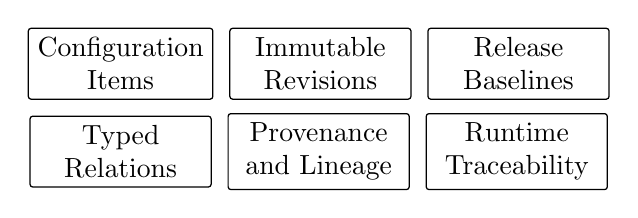
\begin{tikzpicture}[
				baseline,
				component/.style={
					draw,
					rounded corners=1pt,
					minimum width=23mm,
					minimum height=6mm,
					align=center,
					line width=0.45pt
				}
				]
				\node[component] (aci) {Configuration\\Items};
				\node[component, right=2mm of aci] (revisions) {Immutable\\Revisions};
				\node[component, right=2mm of revisions] (baselines) {Release\\Baselines};
				
				\node[component, below=2mm of aci] (relations) {Typed\\Relations};
				\node[component, right=2mm of relations] (provenance) {Provenance\\and Lineage};
				\node[component, right=2mm of provenance] (runtime) {Runtime\\Traceability};
			\end{tikzpicture}
		};
		
		\draw[arrow] (projection) -- (acm);
		
		% ---------------------------------------------------------
		% Governance capabilities
		% ---------------------------------------------------------
		
		\node[layer, below=5mm of acm] (governance) {
			\textbf{Governance Capabilities}\\[4pt]
			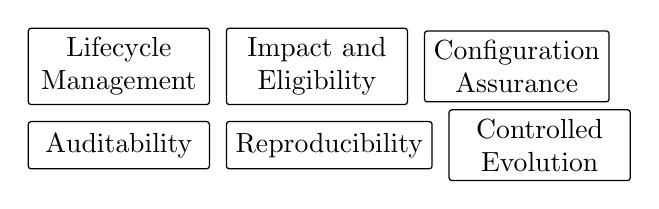
\begin{tikzpicture}[
				baseline,
				component/.style={
					draw,
					rounded corners=1pt,
					minimum width=23mm,
					minimum height=6mm,
					align=center,
					line width=0.45pt
				}
				]
				\node[component] (lifecycle) {Lifecycle\\Management};
				\node[component, right=2mm of lifecycle] (impact) {Impact and\\Eligibility};
				\node[component, right=2mm of impact] (assurance) {Configuration\\Assurance};
				
				\node[component, below=2mm of lifecycle] (audit) {Auditability};
				\node[component, right=2mm of audit] (reproducibility) {Reproducibility};
				\node[component, right=2mm of reproducibility] (change) {Controlled\\Evolution};
			\end{tikzpicture}
		};
		
		\draw[arrow] (acm) -- (governance);
		
	\end{tikzpicture}
	
	\caption{Positioning of ACM with respect to heterogeneous agentic execution frameworks. Native configurations originating from explicit workflow graphs, metadata-driven orchestration, or delegation-based agent systems are semantically projected into a common framework-independent governance representation, allowing lifecycle management, assurance evaluation, provenance, traceability, and controlled evolution to operate independently of the originating execution framework.}
	\label{fig:acm_framework_positioning}
\end{figure}

\subsection{Contributions to Agentic Configuration Governance}
\label{sec:governance_contributions}

The contribution of ACM lies neither in introducing a new orchestration mechanism nor in extending the execution capabilities of existing agentic frameworks. Its primary contribution is to establish configuration governance as an explicit and framework-independent concern for agentic systems. From this perspective, ACM contributes at four complementary levels: representation, semantics, interoperability, and operational validation.

\subsubsection{A Framework-Independent Governance Representation}

The first contribution is a reference model that represents an agentic system as a governed configuration rather than as a collection of framework-specific runtime objects. The model introduces explicit configuration items, immutable revisions, typed relationships, provenance information, and release baselines. These abstractions provide a common vocabulary for describing the constituent elements of an agentic system and the dependencies that determine its effective configuration.

This representation extends established configuration-management principles to artifacts that are specific to agentic systems. In particular, it treats agents, prompts, tools, policies, models, workflows, and dynamically instantiated components as governable objects whose identity and evolution can be tracked independently. The resulting configuration is therefore not reduced to source code, deployment metadata, or execution traces. It is represented as an explicit and auditable object in its own right.

A central consequence of this model is the ability to distinguish logical identity from immutable revision identity. Successive revisions of the same configuration item preserve a stable conceptual identity while remaining individually addressable through exact revision identifiers and content digests. This distinction supports reproducibility, comparison, controlled replacement, and historical reconstruction without conflating an evolving artifact with one of its concrete states.

\subsubsection{Formal Governance Semantics}

The second contribution is the formalization of governance semantics over the reference model. ACM does not merely describe which artifacts exist; it defines how their governance states evolve and how local changes affect dependent configurations.

The lifecycle model specifies admissible transitions for configuration revisions, baselines, and runtime instances. Quality, assurance, impact, and eligibility are maintained as distinct dimensions rather than being collapsed into a single status. This separation prevents ambiguous interpretations such as treating a lack of evidence as proof of poor quality or propagating the lifecycle state of a dependency directly to its parent.

The propagation semantics further define how dependency changes, invalidated evidence, deprecated components, and runtime deviations influence the governance status of composite configurations. These effects are restrictive rather than destructive: a problematic dependency may block the promotion of a composite configuration without rewriting the intrinsic quality or lifecycle state of that composite. The model thereby preserves the provenance of governance decisions while supporting deterministic and explainable state computation.

The assurance model complements these semantics by linking governance conclusions to explicit evidence. Validation and approval are attached to exact revisions and scopes, allowing the system to distinguish directly assessed artifacts from conclusions inherited through assurance-relevant dependencies. Governance states can therefore be interpreted together with the evidence and rules from which they were derived.

\subsubsection{Framework-Independent Semantic Projection}

The third contribution is the separation between framework-specific extraction and framework-independent governance processing. Native configurations are translated into ACM through semantic projection, while the governance kernel operates exclusively on normalized ACM artifacts.

This architecture allows heterogeneous orchestration paradigms to be governed through a common representation. A graph-oriented framework may expose nodes and edges directly, whereas a role- and task-oriented framework may require part of its topology to be reconstructed from assignments and dependencies. ACM does not require these native representations to be structurally identical. It requires the projection to preserve the information needed for configuration governance and to make approximated or unavailable information explicit.

Framework independence should therefore be understood as independence of the governance model and processing semantics from a specific execution framework. The adapters remain framework-specific because they interpret native concepts. Once projection is complete, however, lifecycle validation, baseline construction, dependency analysis, assurance computation, runtime integration, and impact propagation no longer depend on the source framework.

This separation provides a basis for interoperability without imposing a common execution model. Frameworks retain their native orchestration semantics, while ACM supplies a shared governance representation above them.
The experimental evaluation further demonstrates that this interoperability extends beyond heterogeneous orchestration models to heterogeneous introspection regimes. The evaluated frameworks expose governance-relevant information through explicit execution graphs, metadata-assisted reconstruction, and delegation-oriented agent handoffs, respectively. By normalizing these complementary representations into a common ACM configuration graph, semantic projection isolates framework-specific extraction from governance processing, allowing identical governance semantics to be applied independently of the native introspection mechanism.

\subsubsection{Reference Operationalization and Evaluation}

The fourth contribution is the operationalization of the reference model through an executable implementation together with its experimental validation across three representative agentic frameworks. Beyond demonstrating implementability, the reference implementation provides a reproducible operational realization of the proposed governance semantics, including semantic projection, deterministic governance evaluation, runtime reconstruction, and quantitative impact analysis.

The LangGraph, CrewAI, and OpenAI Agents SDK adapters instantiate the semantic-projection boundary for three complementary execution and introspection paradigms. Their diversity does not establish universal applicability, but provides representative evidence that the ACM reference model accommodates heterogeneous configuration abstractions while preserving common governance semantics. 

The evaluation also contributes a structured validation methodology combining normative governance scenarios, automated tests, and semantic-preservation analysis. This methodology distinguishes successful representation from exact structural equivalence and records which governance-relevant properties are preserved, reconstructed, approximated, or unavailable. It therefore provides a more appropriate validation criterion for a reference model than conventional runtime-performance benchmarking. The experimental protocol further complements this qualitative validation with a dedicated quantitative assessment of deterministic impact propagation. Together, the two experimental campaigns demonstrate not only that heterogeneous configurations can be governed through a common reference model, but also that the resulting governance analyses remain reproducible and quantitatively consistent across complementary execution frameworks.

Taken together, these four contributions establish ACM as a configuration-governance abstraction positioned between agentic execution environments and higher-level operational or organizational governance processes. The reference model defines what is governed, the formal semantics define how governance states are computed, semantic projection connects heterogeneous frameworks to the model, and the reference implementation demonstrates that these mechanisms can be operationalized consistently.

\subsection{Practical Implications}
\label{sec:practical_implications}

Beyond its conceptual contribution, ACM has practical implications for the engineering and governance of agentic systems. By introducing an explicit and framework-independent configuration representation, the proposed model enables governance activities that are difficult to perform when configuration information remains fragmented across framework-specific abstractions.

The experimental evaluation indicates that these governance capabilities remain applicable across heterogeneous execution environments despite substantial differences in their native introspection mechanisms. Consequently, governance policies can be formulated over a stable configuration representation rather than being coupled to framework-specific execution abstractions. This separation is particularly important as agentic ecosystems continue to diversify and evolve.

A first implication concerns reproducibility. In current agentic ecosystems, reproducing a previous execution often requires reconstructing configurations from multiple heterogeneous artifacts, including prompts, workflow definitions, deployment parameters, runtime traces, and external resources. ACM addresses this fragmentation by associating executions with immutable configuration revisions and controlled release baselines. A governed execution can therefore be traced back to the exact configuration from which it originated, supporting reproducible experiments, regression analyses, and long-term maintenance. The experimental campaigns further indicate that reproducibility extends beyond immutable configuration snapshots. Equivalent governed representations, deterministic impact propagation, and identical governance outcomes were obtained across repeated executions and heterogeneous execution frameworks. These observations suggest that governance reproducibility depends primarily on the normalized ACM representation rather than on the native execution environment.

A second implication concerns auditability and traceability. Since governance decisions are explicitly linked to identified configuration revisions and supporting evidence, the provenance of a validation result or lifecycle transition becomes inspectable rather than implicit. This capability facilitates post-deployment analysis, compliance reporting, and forensic investigation by making configuration evolution transparent throughout the lifecycle of the system.

The explicit representation of dependencies also supports systematic change management. Instead of reasoning independently about prompts, agents, tools, or models, ACM represents these artifacts as interconnected configuration items whose relationships can be analyzed before modifications are promoted to a released baseline. Dependency-aware impact analysis provides early visibility into the potential consequences of configuration changes, reducing the likelihood of unintended regressions. The quantitative evaluation additionally suggests that governance-driven impact analysis may substantially reduce the configuration space requiring manual verification after a change. Rather than inspecting every potentially affected artifact, practitioners can focus their review on the governed impact set computed through deterministic propagation. Although the reported inspection reduction remains an experimental estimate rather than the outcome of a controlled user study, it illustrates the practical value of combining semantic dependency analysis with explicit governance relationships.


The proposed model also provides a common governance abstraction that may facilitate interoperability across heterogeneous execution environments. Organizations frequently combine multiple orchestration frameworks to address different operational requirements. By projecting these heterogeneous configurations into a shared governance representation, ACM enables governance policies to be expressed independently of the underlying execution technology while allowing each framework to preserve its native execution semantics. 
The evaluation also indicates that interoperability should not be interpreted solely as compatibility between orchestration frameworks. The successful projection of explicit workflow graphs, metadata-assisted orchestration, and delegation-based agent systems suggests that governance interoperability can also be achieved across heterogeneous introspection regimes, provided that governance-relevant semantics are preserved during semantic projection.

ACM may therefore contribute to the emerging AgentOps ecosystem by complementing existing observability and orchestration platforms with explicit configuration governance. Current operational platforms primarily focus on execution monitoring, tracing, evaluation, and operational metrics. ACM addresses a complementary concern by governing the configuration artifacts that determine how those executions are produced. Consequently, the model should be viewed as a governance layer that can coexist with, rather than replace, existing AgentOps and LLMOps infrastructures. 
From this perspective, ACM complements operational observability rather than competing with it. Execution-oriented platforms primarily describe what occurred during runtime, whereas ACM governs the configuration artifacts, dependencies, and assurance evidence that explain why a governed execution was possible. The combination of both perspectives provides a more complete governance foundation spanning configuration, execution, and evolution.

%%%%%%%%%%%%%%%%%%%%%%%%%%%%%%%%%%%%%%%%%%%%%%%%%%%%%%%%%%%%%%%%%%%%%%%%%%%%%%%%
\subsection{Limitations of the Current Reference Model}
\label{subsec:limitations}

The objective of ACM is to provide a framework-independent governance representation for the governance of agentic system configurations rather than an execution platform or an autonomous reasoning architecture. Accordingly, the current version focuses on representing governed configuration artifacts, their lifecycle, dependencies, provenance, assurance, and runtime conformance, while intentionally leaving the internal execution logic of agentic systems outside the scope of the reference model.

Table~\ref{tab:limitations_scope} summarizes the current coverage of ACM and the principal capabilities intentionally deferred to future work.

\begin{table}[t]
	\caption{Current scope of the ACM reference model.}
	\label{tab:limitations_scope}
	\centering
	\begin{tabular}{ll}
		
		\toprule
		
		Currently covered &
		Not yet covered \\
		
		\midrule
		
		Semantic projection &
		Distributed execution \\
		
		Configuration governance &
		Multi-agent planning strategies \\
		
		Immutable revision management &
		Learning and adaptation mechanisms \\
		
		Lifecycle semantics &
		Autonomous reasoning policies \\
		
		Dependency propagation &
		Self-modifying execution strategies \\
		
		Runtime provenance &
		Collective agent negotiation \\
		
		Assurance evaluation &
		Long-term memory management \\
		
		Deterministic replay &
		Continual learning \\
		
		Framework-independent governance &
		Native communication protocols (e.g., MCP, A2A) \\
		
		Cross-framework governance &
		Large-scale industrial validation \\
		
		\bottomrule
		
	\end{tabular}
	
\end{table}

These limitations result from deliberate modeling decisions rather than technical constraints. ACM intentionally separates governance concerns from execution concerns in order to establish a stable and framework-independent governance layer. Integrating planning algorithms, reasoning strategies, learning mechanisms, or execution optimizations into the reference model would both increase its complexity and compromise the conceptual independence required for long-term interoperability.

Consequently, ACM treats reasoning engines, orchestration frameworks, planning modules, learning components, communication protocols, and other execution technologies as external systems whose observable configuration and runtime behavior can be represented and governed without prescribing their internal operation. ACM therefore specifies \emph{what} is governed---configuration revisions, baselines, dependencies, runtime observations, and assurance evidence---rather than \emph{how} autonomous agents reason, plan, negotiate, or learn.

This separation also preserves the stability of the governance model as agentic technologies evolve. New execution frameworks, orchestration paradigms, communication protocols, or reasoning techniques can be incorporated through semantic projection without modifying the governance semantics themselves. The evaluation presented in this paper should therefore be interpreted as validating the ability of ACM to represent and govern heterogeneous agentic configurations, not the correctness, efficiency, or intelligence of the underlying execution mechanisms.

Although the present evaluation demonstrates consistent governance semantics across three representative frameworks, these results should not be interpreted as establishing universal framework coverage. Additional validation across emerging execution environments, communication protocols, and industrial-scale deployments remains necessary to assess the broader applicability of the proposed governance model.

The experimental validation remains limited to the representative orchestration frameworks and configuration scales considered by the reference implementation. Although the reported results provide encouraging evidence regarding the generality of the proposed governance semantics across complementary introspection regimes, they remain confined to controlled experimental scenarios. Broader empirical validation involving additional execution frameworks, industrial-scale configurations, human-centered governance workflows, and emerging agent communication protocols will be required before stronger claims regarding general applicability can be made.

\subsection{Section Summary}

This discussion has positioned ACM as a framework-independent governance layer dedicated to the management of agentic system configurations throughout their lifecycle. Rather than introducing another orchestration framework or execution model, ACM separates governance from execution by providing a common semantic representation upon which lifecycle management, assurance evaluation, dependency analysis, provenance tracking, runtime traceability, and controlled evolution can be performed independently of the originating execution framework.

The experimental evaluation strengthens this positioning by demonstrating that the proposed governance semantics remain applicable across heterogeneous execution frameworks and complementary introspection regimes. Native configurations originating from explicit workflow graphs, metadata-assisted orchestration, and delegation-oriented agent systems are normalized through semantic projection into equivalent governed ACM representations. Together with the quantitative evaluation of deterministic impact propagation, these results indicate that governance can be expressed over a stable and framework-independent configuration model despite substantial differences in native execution abstractions.

The proposed reference model should therefore be viewed as a governance abstraction complementing existing AgentOps and agentic execution ecosystems rather than replacing them. By combining a unified configuration representation with formal governance semantics and reproducible operationalization, ACM establishes a common foundation for configuration governance while remaining intentionally independent of framework-specific orchestration mechanisms. The following section discusses the principal threats to the validity of the present study and the factors that should be considered when interpreting these results.

\bibliographystyle{IEEEtran}
\bibliography{references}
\end{document}

